\documentclass{standalone}
\usepackage[utf8]{inputenc}
\usepackage[T1]{fontenc}
\usepackage[french]{babel}

\usepackage{mathptmx}
\usepackage{tikz}
\usepackage{pgfplots}

\pgfplotsset{compat=newest}
\usetikzlibrary{positioning}

\begin{document}
	\usetikzlibrary{positioning}
\begin{tikzpicture}



\begin{axis}[
	 axis lines=left, 
	 xtick=\empty,
	 ytick=\empty,
	 width=0.9\textwidth,
     xmin=0,xmax=4,
     ymin=0,ymax=4,
	 xlabel=Temps simulé,
	 every axis x label/.style={at={(ticklabel* cs:1.02)},anchor=north},
	 ylabel=Taille des objets,
	 ylabel style={rotate=-90},
	 every axis y label/.style={at={(ticklabel* cs:1.02)},anchor=south,},
	 extra y ticks={1,2,3},
	 extra y tick labels={Atome, Grain, Solide}
	 ]
     
     \node (A) at (axis cs:0.9,0.9) [label={[align=center]below:\textbf{Dynamique Moléculaire}\\Terentyev et. al.}] {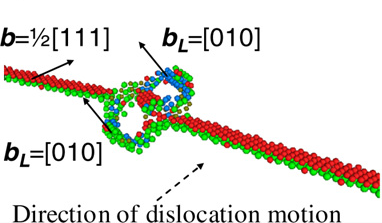
\includegraphics[height=0.15\textwidth]{img/comparaison-xshi-md}};
     \node (B) at  (axis cs:2,2) [label={[align=center]below:\textbf{Dynamique des Dislocations}\\OptiDis}] {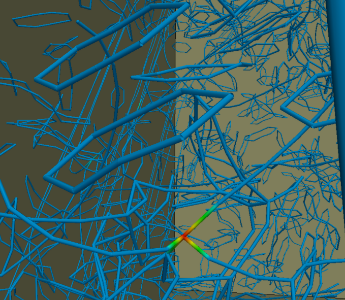
\includegraphics[height=0.15\textwidth]{img/multiscale-dd}};
     \node (C) at (axis cs:3,3) [label={[align=center]below:\textbf{FFT}\\Amitex-FFTP}] {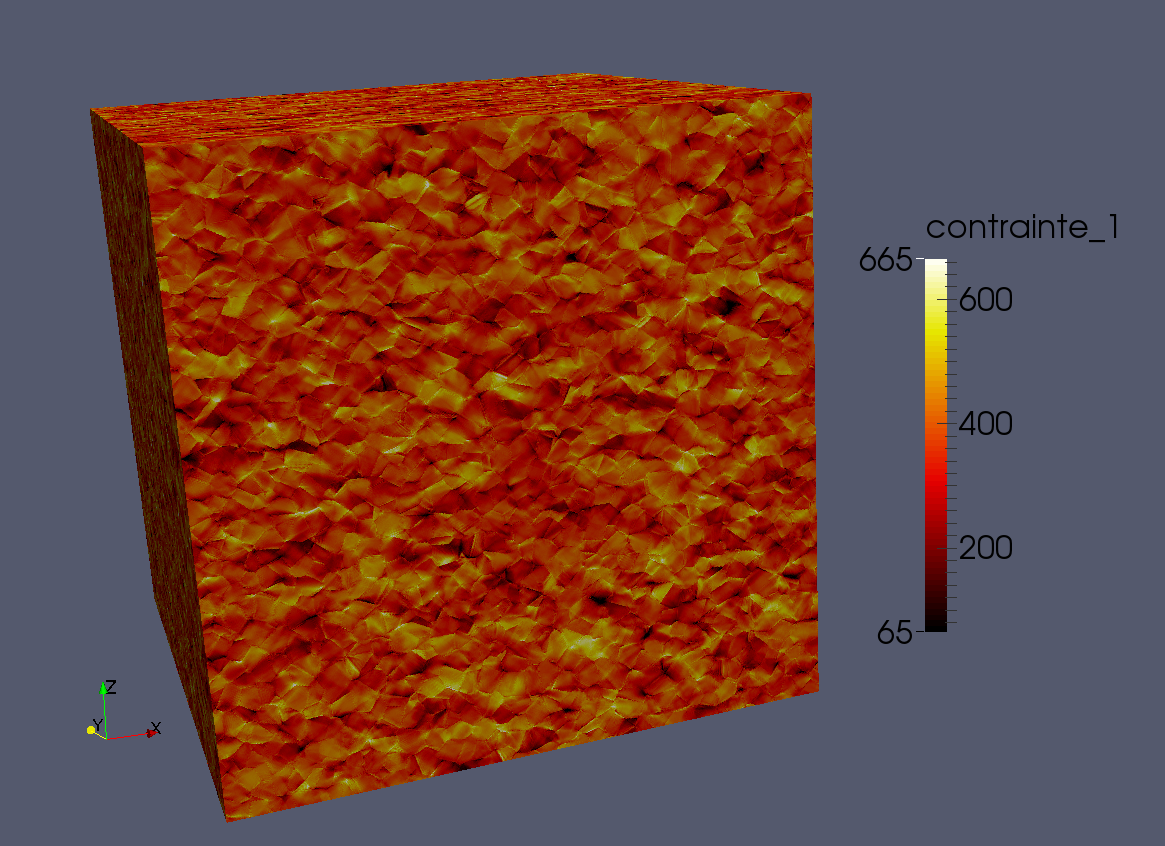
\includegraphics[height=0.15\textwidth]{img/amitex-fftp}};
    \node [left = of A] (D) {};
    \node [above = of C] (E) {};
    \draw[thick, ->] (D) to [bend left] (E);

 \end{axis} 
 
\end{tikzpicture}
\end{document}